\documentclass[border=4pt]{standalone}
\usepackage{pgfplots}
\pgfplotsset{compat=1.18}

\begin{document}
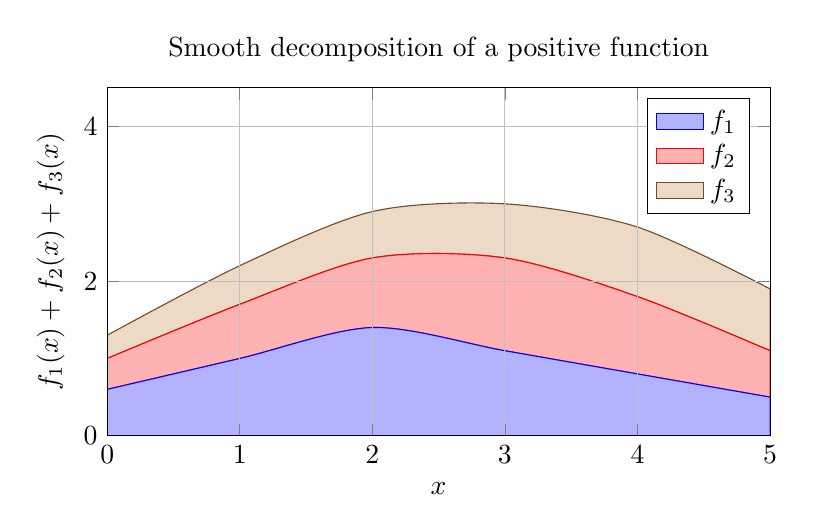
\begin{tikzpicture}
  \begin{axis}[
    smooth,
    stack plots=y,
    area style,
    width=10cm,
    height=6cm,
    xmin=0,
    xmax=5,
    ymin=0,
    ymax=4.5,
    enlargelimits=false,
    xlabel={$x$},
    ylabel={$f_1(x)+f_2(x)+f_3(x)$},
    title={Smooth decomposition of a positive function},
    grid=major,
    legend pos=north east
  ]
    \addplot coordinates {(0,0.6) (1,1.0) (2,1.4) (3,1.1) (4,0.8) (5,0.5)} \closedcycle;
    \addplot coordinates {(0,0.4) (1,0.7) (2,0.9) (3,1.2) (4,1.0) (5,0.6)} \closedcycle;
    \addplot coordinates {(0,0.3) (1,0.5) (2,0.6) (3,0.7) (4,0.9) (5,0.8)} \closedcycle;
    \legend{$f_1$,$f_2$,$f_3$}
  \end{axis}
\end{tikzpicture}
\end{document}
